\documentclass[border=10pt]{standalone}
\usepackage{tikz}
\usepackage{amsmath}
\usetikzlibrary{shadows}

\begin{document}

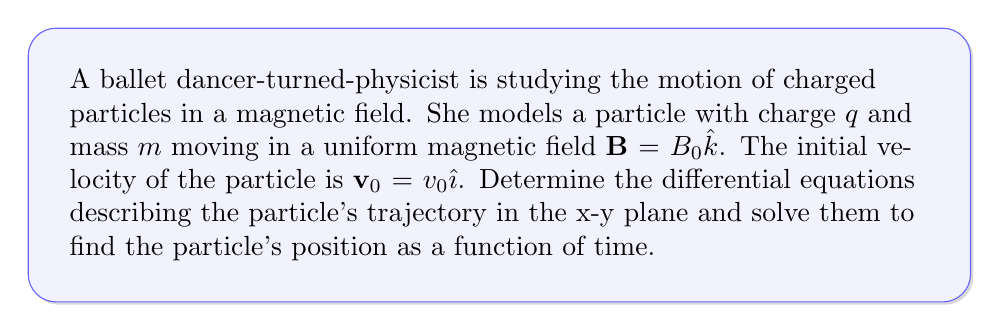
\begin{tikzpicture}
\node[draw=blue!60, fill=blue!5, text width=0.9\textwidth, 
      align=left, rounded corners=10pt, 
      inner sep=15pt, drop shadow={shadow xshift=1pt, shadow yshift=-1pt, opacity=0.3}]
{
A ballet dancer-turned-physicist is studying the motion of charged particles in a magnetic field. She models a particle with charge $q$ and mass $m$ moving in a uniform magnetic field $\mathbf{B} = B_0 \hat{k}$. The initial velocity of the particle is $\mathbf{v}_0 = v_0 \hat{\imath}$. Determine the differential equations describing the particle's trajectory in the x-y plane and solve them to find the particle's position as a function of time.
};
\end{tikzpicture}

\end{document}